\documentclass{beamer}
\usetheme{metropolis}
\usecolortheme{seahorse}
\setbeamertemplate{frame numbering}[fraction]
\metroset{block=fill}

\usepackage[utf8]{inputenc}

\usepackage{graphicx}
\graphicspath{ {./imgs/} }

\usepackage{multicol}

\usepackage{soul} % strikethrough


\title{We Have Built Nice Things}
\subtitle{Ossification is not Stagination}
\author{Wang, Hao (she / her)}
\institute{Lead Software Architect @ Graveflex | ms-jpq @ github | hola@bigly.dog}
\date{}


\begin{document}


\begin{frame}

	\titlepage

\end{frame}


\begin{frame}{Correction}

	Wrong employer on speakers list

	\rule{\textwidth}{0.1em}

	Lead Engineer @ \textit{\textbf{Sun}Cloud} not \textit{\textbf{Sound}Cloud}

\end{frame}


\begin{frame}{\$NEW\_JOB}

	Lead Software Architect @ Graveflex

	\rule{\textwidth}{0.1em}

	\begin{center}

		
\includegraphics[width=16em,height=16em]{graveflex}

	\end{center}

\end{frame}


\begin{frame}{about:me}

	\rule{\textwidth}{0.1em}

	\begin{itemize}

		\begin{multicols}{2}

			\item CHADTree

			File manager

			\hspace{0.1em}

			\item COQ.nvim

			Auto completion

			\hspace{0.1em}

			\item sad

			Batch regex edits (TUI)

			\hspace{0.1em}

			\item lua async await

			Concurrency library

			\hspace{0.1em}

		\end{multicols}

	\end{itemize}

	\rule{\textwidth}{0.1em}

\end{frame}


\begin{frame}{Inspiration}

	We can have nice things - \textit{Justin M. Keyes}

	\vspace{1em}

	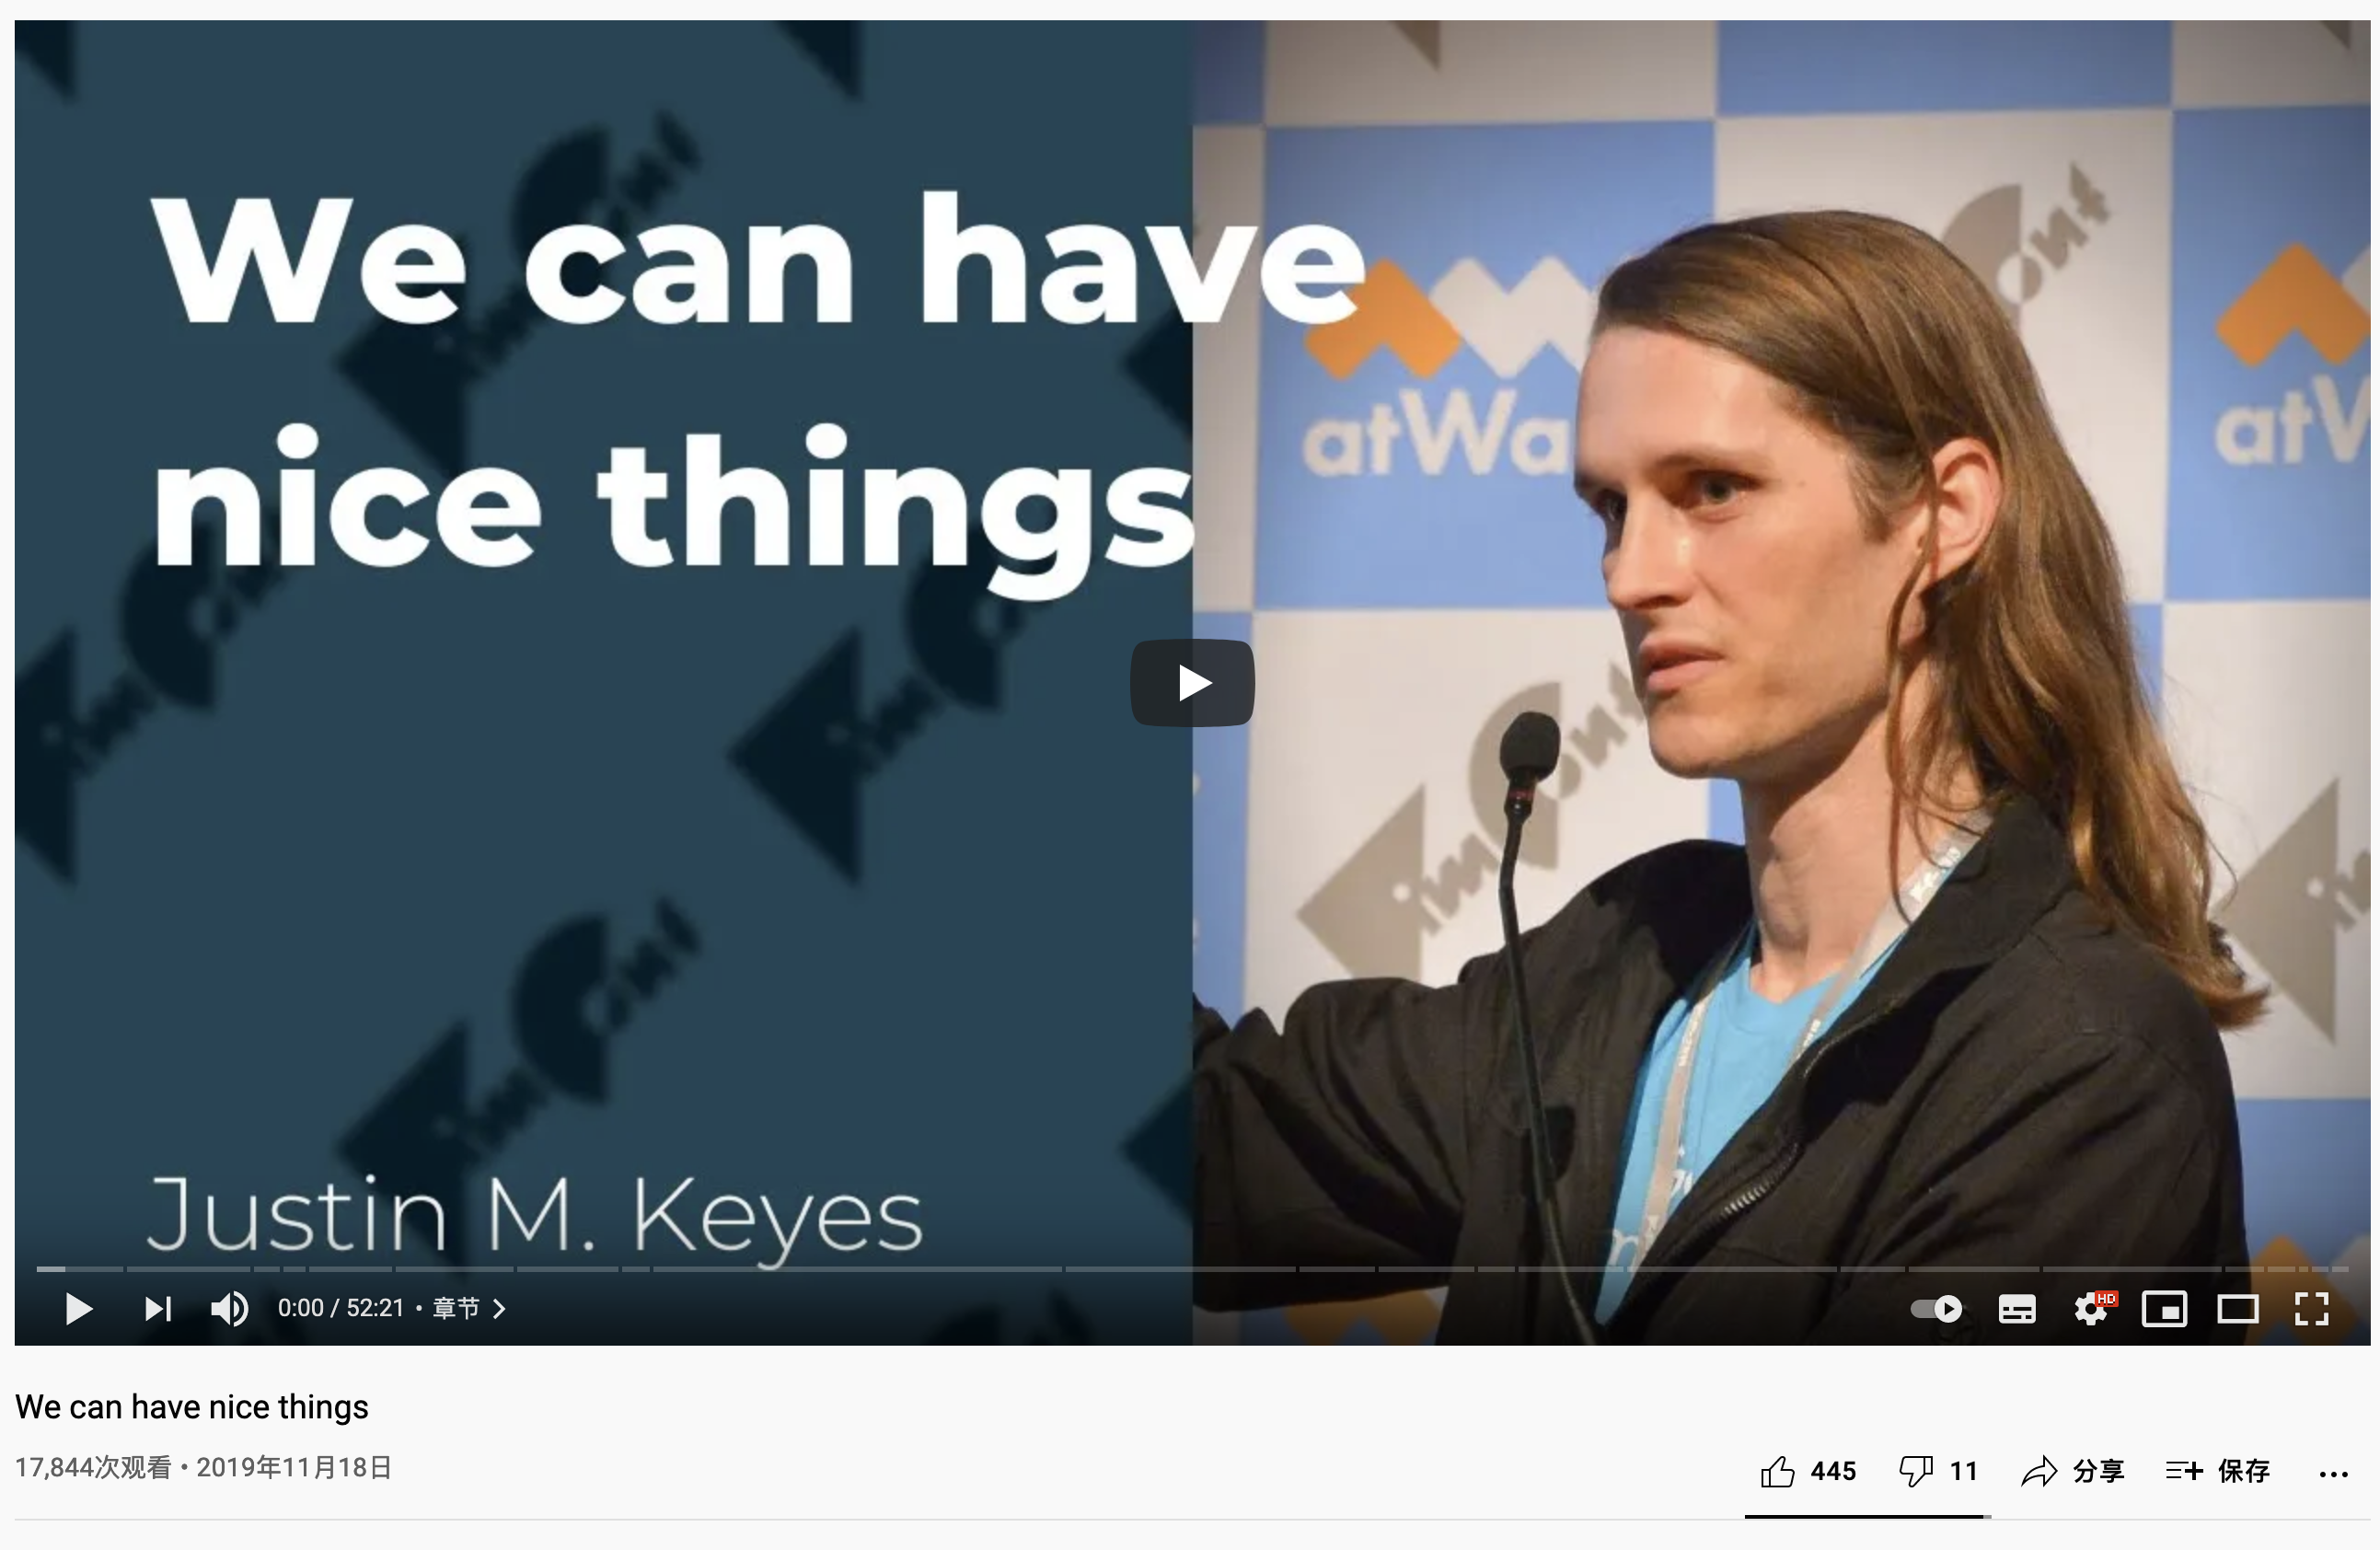
\includegraphics[width=\textwidth]{we_can_have_nice}

\end{frame}


\begin{frame}{Ossification -> Innovation}

	\textbf{Ossofication is not Stagnation}

	\rule{\textwidth}{0.1em}

	\begin{itemize}

		\item Nvim has comes with a historied legacy

		\item Consequences of legacy

		\item Gifts of legacy

	\end{itemize}

\end{frame}


\begin{frame}[standout]

	Ossification of Ecosystem

	(Existing Plugins)

\end{frame}


\begin{frame}{Vim "philosophy"}

	Driver of ossification

	\rule{\textwidth}{0.1em}

	\begin{itemize}

		\begin{multicols}{2}

			\item unix-y

			\item ad hoc

			\item macro driven

			\item minimalist

			\item extensible

			\item composible

			\item conservative

			\item worse is better

		\end{multicols}

	\end{itemize}

\end{frame}


\begin{frame}{Weight of History}

	\begin{itemize}

		\begin{multicols}{2}

			\item slowiness

			\item jankiness

			\item ossification

			\item interlocking

			\item beginner hostile

			\item dx hostile

		\end{multicols}

	\end{itemize}

\end{frame}


\begin{frame}[standout]

	Ossification of User Habits

\end{frame}


\begin{frame}{Inertia}

	Reverence for the \textit{status quo}

	\rule{\textwidth}{0.1em}

	People want a faster horse.

	Faster horse not good enough to break habits.

	\rule{\textwidth}{0.1em}

	Need \textbf{\textit{significant value proposition}}.

\end{frame}


\begin{frame}{Tolerance for Heresy}

	User mindset

	\rule{\textwidth}{0.1em}

	\begin{itemize}

		\item Fork the codebase

		\item Fork the community

		\item Fork the culture

	\end{itemize}

\end{frame}


\begin{frame}[standout]

	Have Your Cake and Eat It Too

	\textbf{Don't expose implementations}

	\textit{Extensibility still possible}
\end{frame}


\begin{frame}{AOT Static Linking}

	\st{Web} Vim Scrapping

	\rule{\textwidth}{0.1em}

	"Zero runtime cost" -- \st{rust} JSON

	\begin{enumerate}

		\item Compile \text{existing plugins} for artifacts

		\item Dump them into a static file

	\end{enumerate}

\end{frame}


\begin{frame}{Ossification -> Unofficial API}

	"Compiler" can perform validation too!

	\rule{\textwidth}{0.1em}

	\begin{itemize}

		\item CHADTree

		      \begin{itemize}

			      \item 3 icon themes

			      \item 9 colour themes

			      \item 700+ language colours

		      \end{itemize}

		\item COQ.nvim

		      \begin{itemize}

			      \item 13,000+ snippets

			      \item \textbf{zero runtime parse errors}

		      \end{itemize}

	\end{itemize}

\end{frame}


\begin{frame}{Dynamic Linking}

	Can't just AOT everything

	\rule{\textwidth}{0.1em}

	What about runtime interface?

\end{frame}


\begin{frame}{Ossification Kills}

	Notice a pattern here:

	\begin{itemize}

		\item nvim-completion-manager -> ncm2

		\item neocomplete.vim -> deoplete.nvim -> ddc.vim

		\item nvim-compe -> nvim-cmp

		\item completion-nvim -> \st{still ok!} \textit{archived}

	\end{itemize}

	Too big to rewrite:

	\begin{itemize}

		\item YouCompleteMe

		\item coc.nvim

	\end{itemize}

\end{frame}


\begin{frame}[standout]

	Move Fast Without Breaking Things

\end{frame}


\begin{frame}{Protocols are \textbf{meant to be ossified}}

	Implementations are not

	\rule{\textwidth}{0.1em}

	Some protocols are \textit{accidental} or \textit{emergent}

	\begin{itemize}

		\item vim.bo.omnifunc

		\item :h complete-items

		\item \textbf{LSP}

	\end{itemize}

\end{frame}


\begin{frame}{Zero Public Code}

	\begin{enumerate}

		\item Third party code \textbf{CAN NOT} call into coq.nvim

		\item They register callbacks at well known locations (Vim Tradition)

		\item Callbacks communicate via LSP

	\end{enumerate}

\end{frame}


\begin{frame}{PaaS}

	What is the platform

	\rule{\textwidth}{0.1em}

	\begin{itemize}

		\item Your app is not the \textbf{platform}

		\item Nvim is the \textbf{platform}

		\item Ecosystem is the \textbf{platform}

	\end{itemize}

	\rule{\textwidth}{0.1em}

	Nvim :: Browser for the TUI

\end{frame}


\begin{frame}{\$LS\_COLORS}

	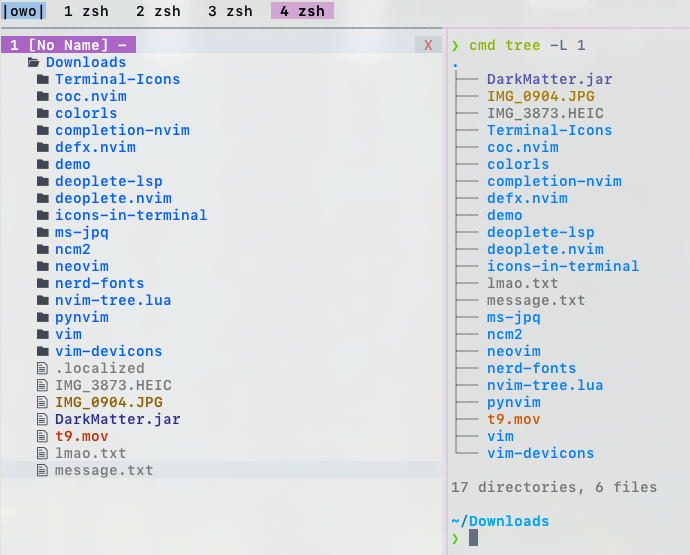
\includegraphics[width=\textwidth,height=20em]{chadtree_ls}

\end{frame}


\begin{frame}[standout]

	When to Break Traditions

\end{frame}


\begin{frame}{Worse is Not Always Better}

	Worse is better for \textbf{software} not \textbf{wetware}

	\rule{\textwidth}{0.1em}

	\begin{itemize}

		\item Computers fast

		\item Meatbags slow

	\end{itemize}

	\rule{\textwidth}{0.1em}

	\st{Implementations Simplicity} Humans are not computers

\end{frame}


\begin{frame}{Humans Suck}

	Designing for meatbags.

	\rule{\textwidth}{0.1em}

	\begin{block}{Observations}

		\begin{itemize}

			\item Computers are \textit{fast}, humans are \textit{slow}

			\item Humans can't typo good

			\item Humans have low working memory

		\end{itemize}

	\end{block}

	\rule{\textwidth}{0.1em}

	Example: Drop requirement for exact prefix match for completions

\end{frame}


\begin{frame}{Data Driven Completion Ranking}


	Link to 2 stage algorithm

	Robust against 2 character typos\footnote{except in first 2 characters}

	https://github.com/ms-jpq/coq\_nvim/blob/coq/docs/FUZZY.md

	\rule{\textwidth}{0.1em}

	Borrow ideas from ML's data processing

	Weights, normalization \& sigmoid func adjust for user inputs

\end{frame}


\begin{frame}[standout]

	Showcase

	(if we have time)

\end{frame}


\begin{frame}{Both::Config Parser}

	Type checker for plugin configuration

	\rule{\textwidth}{0.1em}

	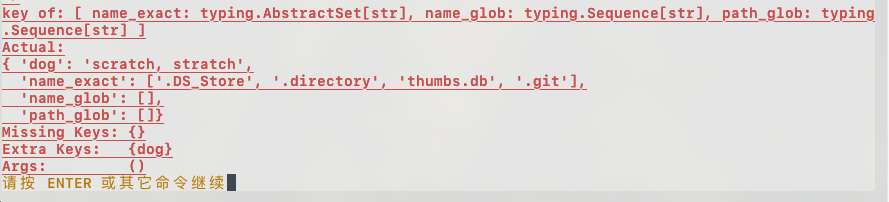
\includegraphics[width=\textwidth]{conf_parser}

	Warns for unnecessary "dog" key

\end{frame}


\begin{frame}{COQ::Snippet REPL}

	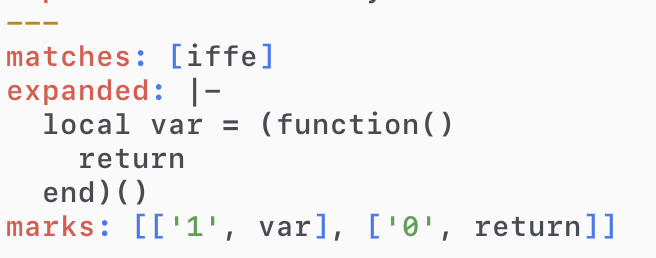
\includegraphics[width=\textwidth]{repl_succ}

	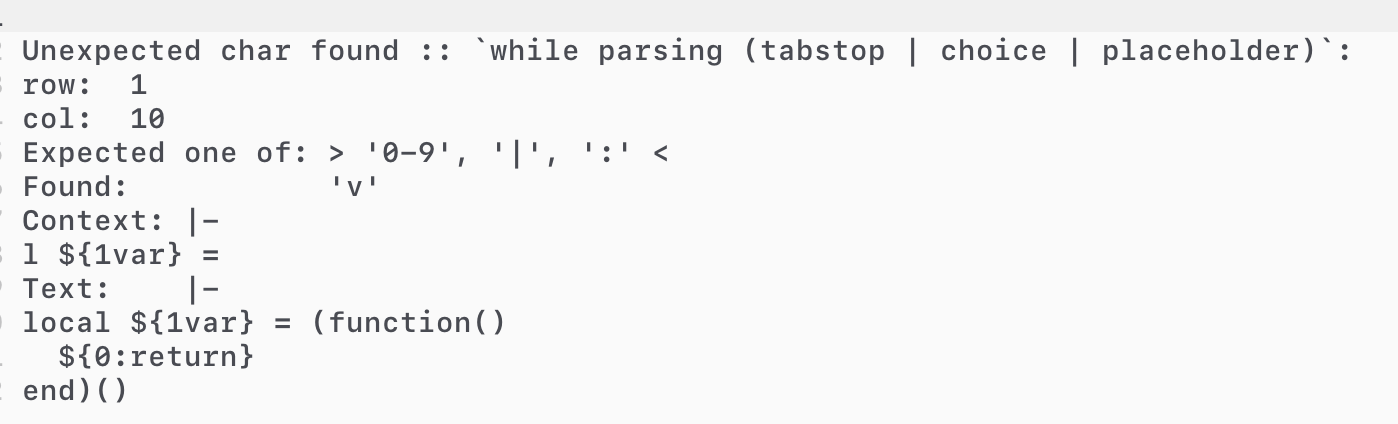
\includegraphics[width=\textwidth]{repl_fail}

\end{frame}


\begin{frame}{COQ::Stats}

	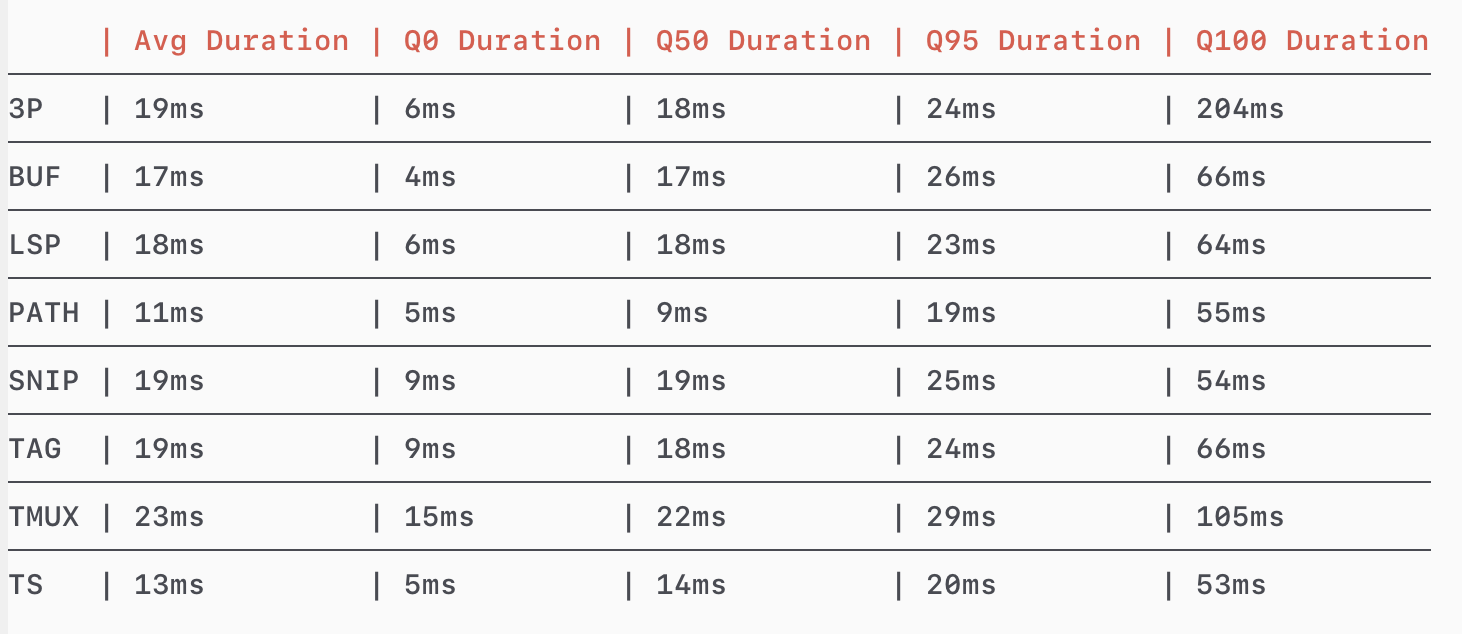
\includegraphics[width=\textwidth]{stats}

\end{frame}


\begin{frame}{Sad::Substitution}

	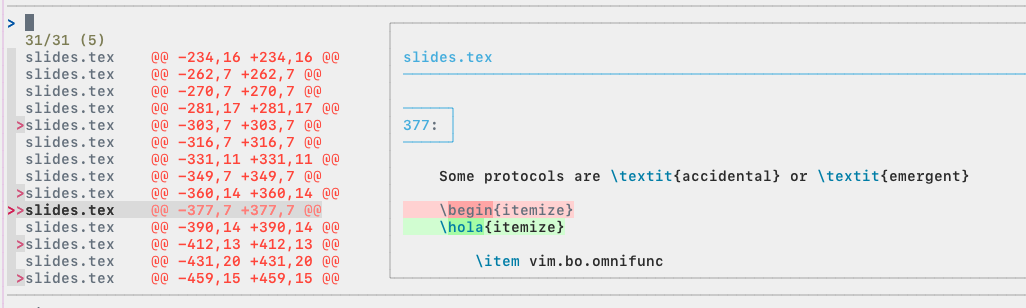
\includegraphics[width=\textwidth]{sad}

\end{frame}


\begin{frame}{Tying the Knot}

	\begin{centering}

		{\Large Technical Factors $\cup$ Cultural Factors}

		\rule{\textwidth}{0.1em}

		{\LARGE Nice things}

	\end{centering}

\end{frame}


\begin{frame}[standout]

	Q \& A

\end{frame}


\end{document}
